\documentclass{article}
\usepackage{amsmath}
\usepackage{amsthm}
\usepackage{amssymb}
\usepackage{amsfonts}
\usepackage{dsfont}
\usepackage{enumerate}
\usepackage{hyperref}
\usepackage{amsmath,color}
\usepackage{graphicx}
\usepackage{booktabs}
\usepackage[table,xcdraw]{xcolor}
\newcommand{\eqsp}{\,}

\graphicspath{ {images/} }


\title{End-to-end deep metamodeling to calibrate and optimize energy loads - Supplementary material}

\begin{document}
\maketitle

\section{Dataset}
\subsection{Inputs}
The dataset is divided in four sub-variables, each representing a different aspect of the simulation. When creating the dataset using the Building Energy Model (here TRNSYS), we sampled each variable uniformly in a given interval. These intervals  are also used for the calibration process.

\begin{enumerate}[-]
    \item $\theta_{building}$ represents the geometric properties of the building, see Table~\ref{tab:theta-building}.
    \item $I_k$ stores the schedules and settings of the heating and ventilation, see  Table~\ref{tab:Ik}. This is the only parameter tuned during the optimization process.
    \item $O_k$ stores the occupation schedules of the building, see Table~\ref{tab:Ok}. These values are calibrated to match real data, and kept fixed during the optimization.
    \item $W_k$ stores the weather data for the week, see Table~\ref{tab:Wk}. In this paper, we exclusively use data collected by weather institutes, that are available afterward. In practice, these data would be replaced by weather forecasts.
\end{enumerate}

The distribution of the outdoor temperature can be found in Figure~\ref{fig:dataset_input_distribution}. We sampled a total of 40 000 examples for our dataset, of which 38 000 were used for training, 1 000 for validation and 1000 for testing purposes.

\begin{figure}
    \centering
    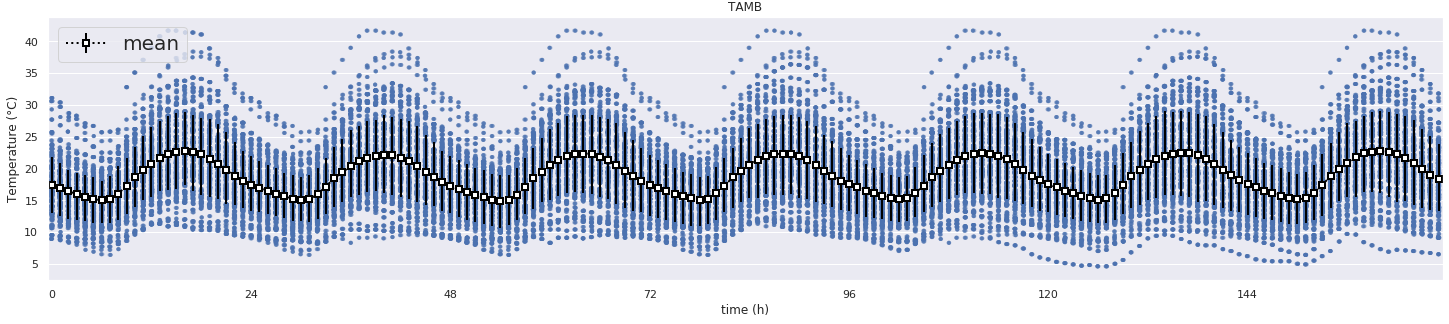
\includegraphics[width=\textwidth]{dataset_distribution_Z_168h.png}
    \caption{Distribution of the outdoor temperature in the dataset, stored in the \texttt{T\_AMB} variable in the Table~\ref{tab:Wk}. Squares indicates the mean value, while vertical bars represent 85\% of the data.}
    \label{fig:dataset_input_distribution}
\end{figure}

\begin{table}
	\centering
	\begin{tabular}{@{}llll@{}}
		Variable                             & Minimum & Maximum & Step \\ \midrule
		airchange\_infiltration\_vol\_per\_h & 0.1     & 0.5     & 0.1  \\
		capacitance\_kJ\_perdegreK\_perm3    & 50      & 300     & 10   \\
		power\_VCV\_kW\_heat                 & 0       & 1000    & 100  \\
		power\_VCV\_kW\_clim                 & 0       & 1000    & 100  \\
		nb\_occupants                        & 1000    & 2000    & 200  \\
		nb\_PCs                              & 1000    & 2000    & 200  \\
		percent\_light\_night                & 0       & 70      & 10   \\
		percent\_PCs\_night                  & 0       & 70      & 10   \\
		facade\_1\_thickness\_2              & 0.05    & 0.15    & 0.05 \\
		facade\_2\_thickness\_2              & 0.05    & 0.15    & 0.05 \\
		facade\_3\_thickness\_2              & 0.05    & 0.15    & 0.05 \\
		facade\_4\_thickness\_2              & 0.05    & 0.15    & 0.05 \\
		roof\_1\_thickness\_3                & 0.05    & 0.15    & 0.05 \\
		facade\_1\_window\_area\_percent     & 40      & 50      & 5    \\
		facade\_2\_window\_area\_percent     & 40      & 50      & 5    \\
		facade\_3\_window\_area\_percent     & 40      & 50      & 5    \\
		facade\_4\_window\_area\_percent     & 40      & 50      & 5    \\
		\bottomrule                                                     \\
	\end{tabular}
	\caption{$\theta\_buidling$ ranges.}
	\label{tab:theta-building}

\end{table}

\begin{table}
	\centering
	\begin{tabular}{@{}llll@{}}
		Variable                & Minimum & Maximum & Step \\ \midrule
		start\_clim\_day        & 7       & 9       & 1    \\
		end\_clim\_day          & 18      & 20      & 1    \\
		t\_clim\_red\_day       & 24      & 30      & 0.5  \\
		t\_clim\_conf\_day      & 20      & 24      & 0.5  \\
		start\_heat\_day        & 6       & 8       & 1    \\
		end\_heat\_day          & 17      & 19      & 1    \\
		t\_heat\_red\_day       & 17      & 22      & 0.5  \\
		t\_heat\_conf\_day      & 22      & 24      & 0.5  \\
		start\_ventilation\_day & 7       & 9       & 1    \\
		end\_ventilation\_day   & 18      & 20      & 1    \\
		t\_ventilation\_day     & 18      & 26      & 0.5  \\
		vol\_ventilation\_day   & 0.7     & 1.7     & 0.3  \\
		\bottomrule                                        \\
	\end{tabular}
	\caption{$I_k$ ranges. Each parameter can hold a different value for each day of the week. For ease of reading, we replaced them by a single line, as the ranges are the same for every day.}
	\label{tab:Ik}

\end{table}

\begin{table}
	\centering
	\begin{tabular}{@{}llll@{}}
		Variable                     & Minimum & Maximum & Step \\ \midrule
		start\_occupation\_monday    & 7       & 9       & 1    \\
		start\_occupation\_tuesday   & 7       & 9       & 1    \\
		start\_occupation\_wednesday & 7       & 9       & 1    \\
		start\_occupation\_thursday  & 7       & 9       & 1    \\
		start\_occupation\_friday    & 7       & 9       & 1    \\
		end\_occupation\_monday      & 17      & 20      & 1    \\
		end\_occupation\_tuesday     & 17      & 20      & 1    \\
		end\_occupation\_wednesday   & 17      & 20      & 1    \\
		end\_occupation\_thursday    & 17      & 20      & 1    \\
		end\_occupation\_friday      & 17      & 20      & 1    \\
		\bottomrule                                             \\
	\end{tabular}
	\caption{$O_k$ ranges.}
	\label{tab:Ok}
\end{table}

\begin{table}
	\centering
	\begin{tabular}{*2c}
		Variable & Description                    \\ \midrule
		DNI      & Direct Normal Irradiance       \\
		IBEAM\_H & Direct Horizontal Irradiance   \\
		IBEAM\_N & Direct Normal Irradiance       \\
		IDIFF\_H & Diffuse Horizontal Irradiation \\
		IGLOB\_H & Global Horizontal Irradiance   \\
		RHUM     & Humidity                       \\
		TAMB     & Outdoor temperature            \\
		\bottomrule                               \\
	\end{tabular}
	\caption{Weather data as contained in $W_k$.}
	\label{tab:Wk}
\end{table}

\subsection{Outputs}
The BEM outputs 8 simulated variables at each time step, representing inside temperature as well as various consumption. These variables are aggregated differently during calibration and optimization. Since the metamodel aims at replicating the BEM behavior, it is trained to output these same 8 variables. See Table~\ref{tab:output_variables} for a exhaustive list and description of each one. Their distributions in the dataset can be found in Figure~\ref{fig:dataset_output_distribution}.

\begin{figure}
    \centering
    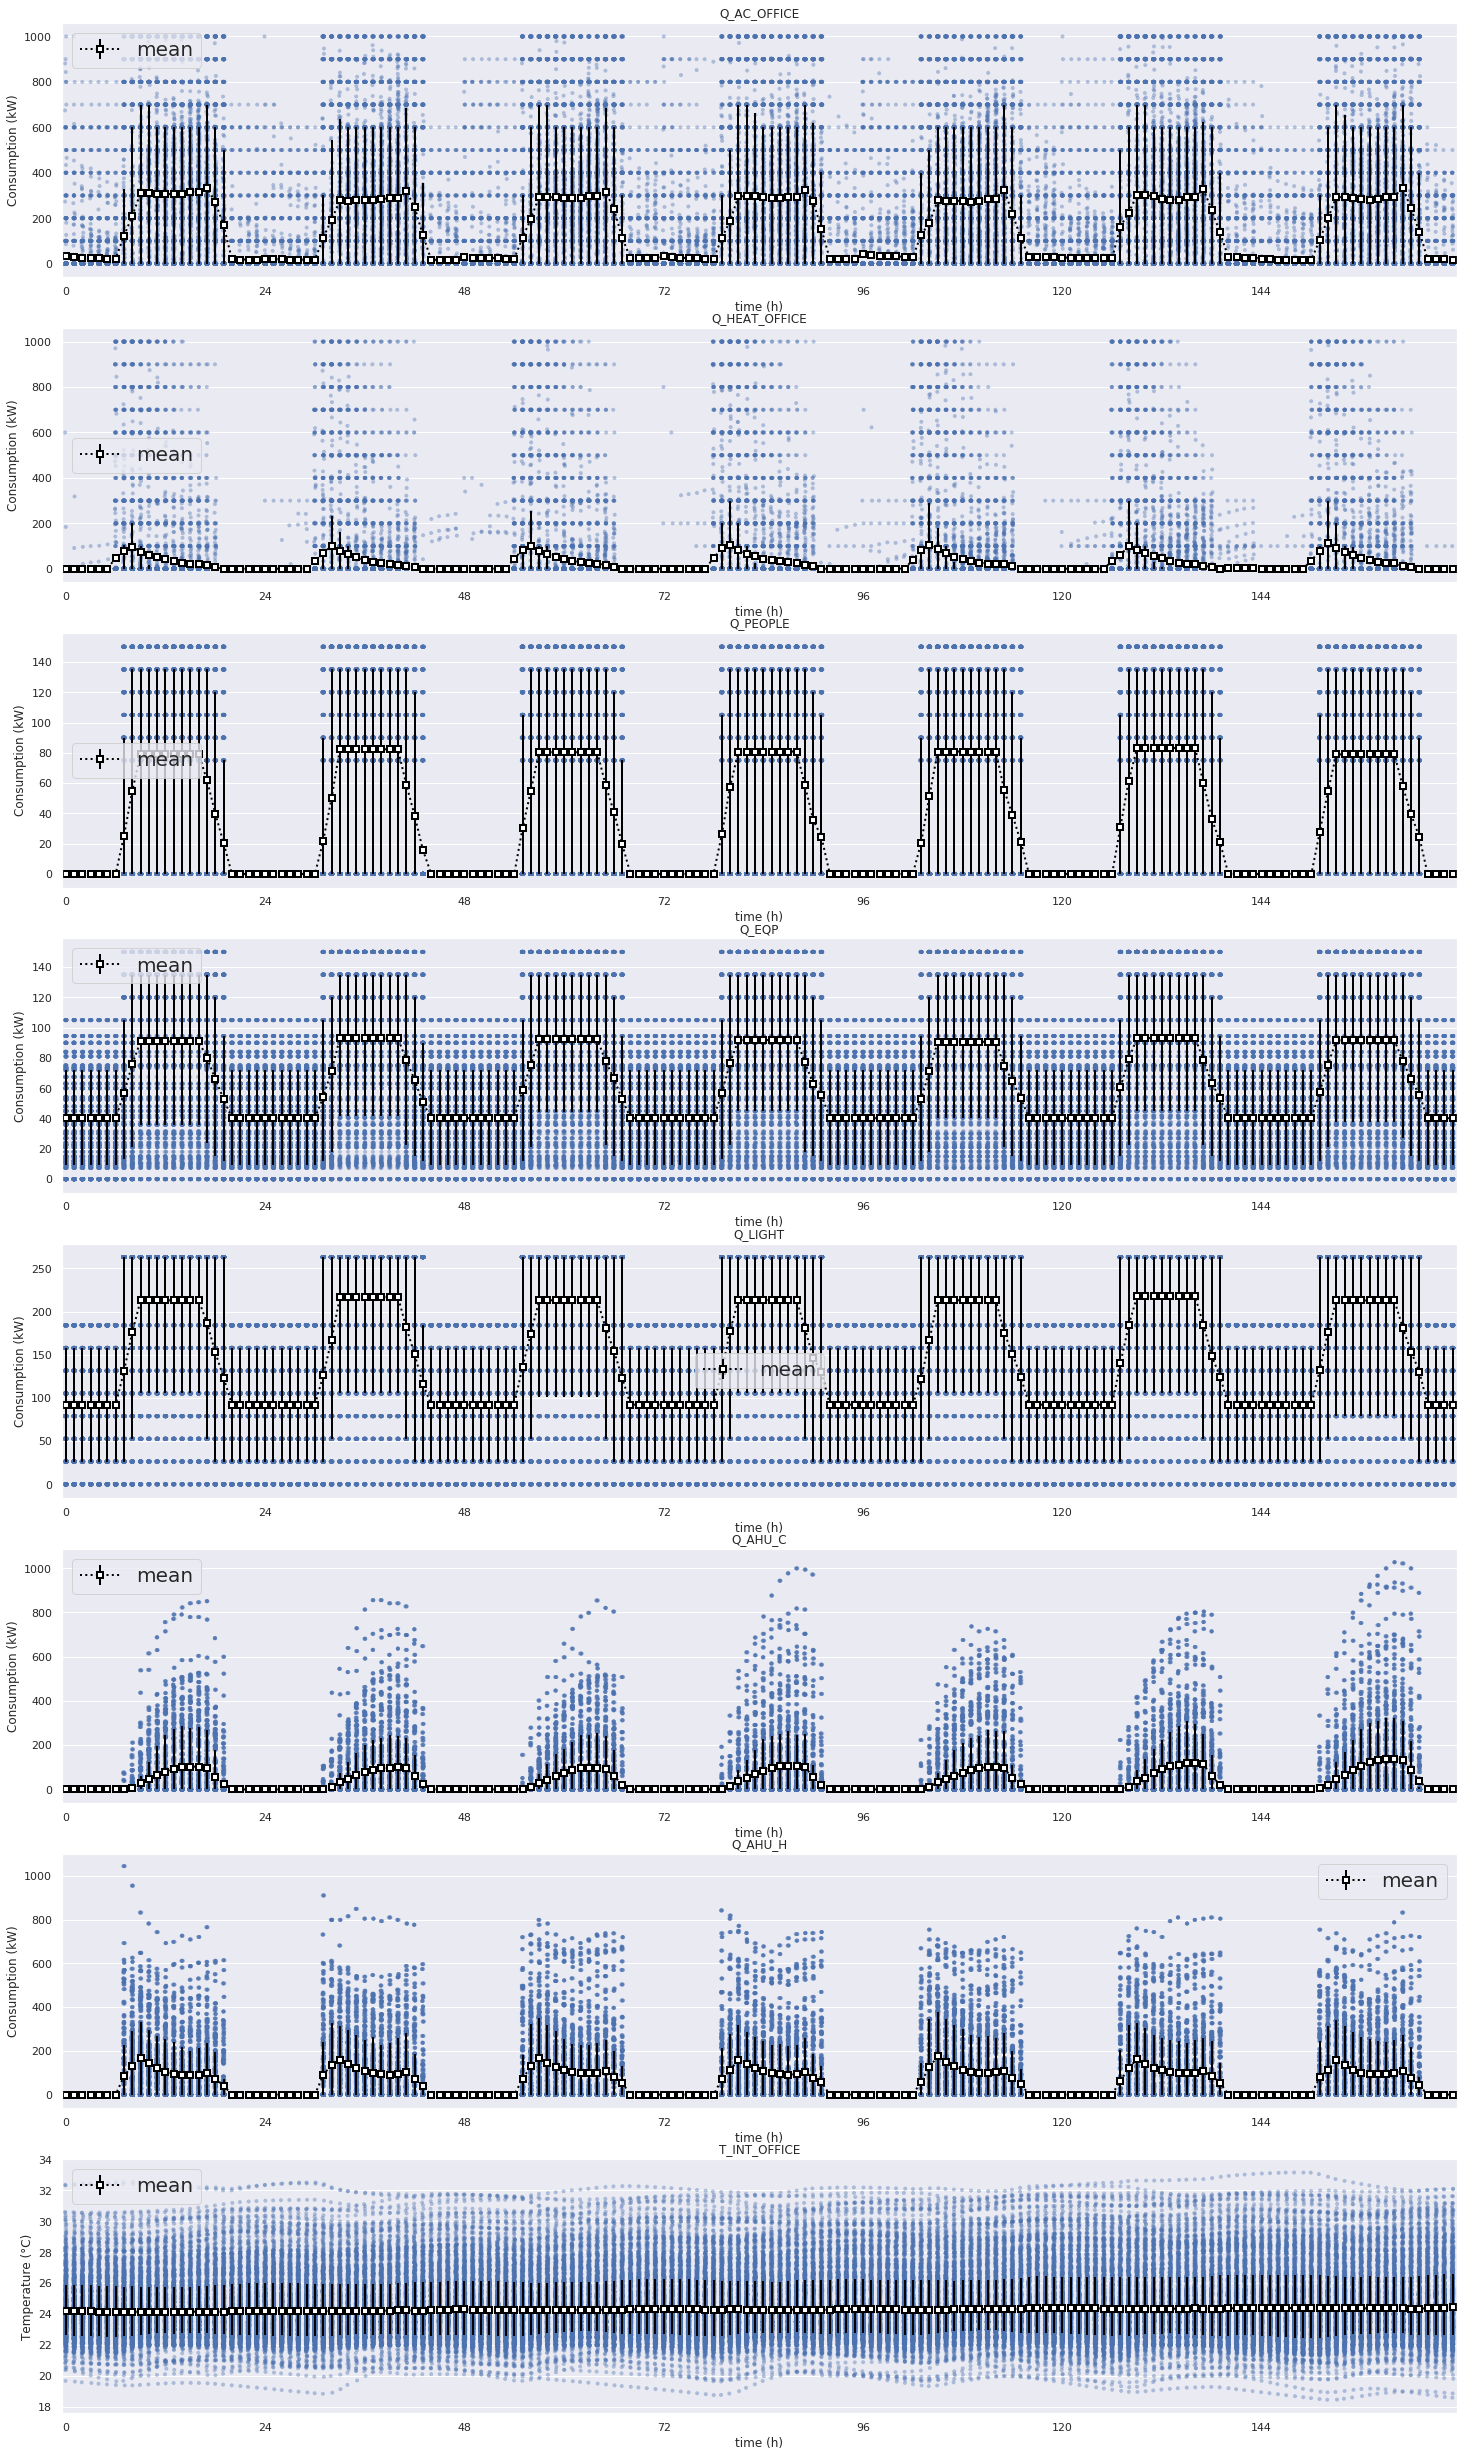
\includegraphics[width=0.95\textwidth]{dataset_distribution_X_168h.png}
    \caption{Distribution of the output variables of the BEM. See Table~\ref{tab:output_variables} for a exhaustive list and description of each one. Squares indicates the mean value, while vertical bars represent 85\% of the data.}
    \label{fig:dataset_output_distribution}
\end{figure}


\section{Metamodel training}
In order to find an optimal set of hyper parameters, we conducted a grid search for the Transformer model. A list of each parameter, along with its ranges and final value, can be found in Table~\ref{tab:grid_search}.

\begin{table}
    \centering
    \begin{tabular}{*3c}
        Variable                                     & Tested values   & Chosen value \\ \midrule
        Latent dimension ($d_{emb}$)                 & 16, 32, 64, 128 & 64           \\
        Queries ($W^q$) and Keys ($W^k$) matrix size & 4, 8, 16        & 8            \\
        Values ($W^v$) matrix size                   & 4, 8, 16        & 8            \\
        Number of heads ($h$)                        & 4, 8, 16        & 8            \\
        Number of layers ($N$)                       & 4, 8, 16        & 4            \\
        Attention size ($\Delta$)                    & 6, 12, 24       & 12           \\
        \bottomrule                                                                   \\
    \end{tabular}
    \caption{Hyper parameters tuned during grid search, along with their tested and chosen values.}
    \label{tab:grid_search}
\end{table}

\section{Calibration}
Sensors installed in the building yield two time series.
\begin{itemize}
    \item \textbf{Indoor temperature}: we average the values from a set of sensors, in order to obtain a unique indoor temperature value at each time step. This temperature is compared to the simulated indoor temperature (\texttt{T\_INT}).
    \item \textbf{Heat consumption}: we define building heat consumption as the sum of multiple private heat consumptions obtained from sensors. This variable contains the heating consumption (corresponding to \texttt{Q\_HEAT\_OFFICE} for the metamodel), as well as the heating AHU consumption (\texttt{Q\_AHU\_HEAT}), and the equipment and lighting consumption (\texttt{Q\_EQP} and \texttt{Q\_LIGHT} respectively), see Table~\ref{tab:output_variables} for a description of the metamodel output variables. These four simulated variables are summed and compared to the real heat consumption.
\end{itemize}

\begin{table}
	\centering
	\begin{tabular}{@{}llll@{}}
		variable        & description                                     \\ \midrule
		Q\_AC\_OFFICE   & AC consumption                                  \\
		Q\_HEAT\_OFFICE & Heat consumption                                \\
		Q\_PEOPLE       & Heating power from human activities             \\
		Q\_EQP          & Equipment (computers, elevators, fridges, etc.) \\
		Q\_LIGHT        & Consumption of lights                           \\
		Q\_AHU\_C       & Consumption of AHU when cooling outside air     \\
		Q\_AHU\_H       & Consumption of AHU when heating outside air     \\
		T\_INT\_OFFICE  & Indoor temperature                              \\
		\bottomrule                                                       \\
	\end{tabular}
	\caption{BEM's output variables at each time step.}
	\label{tab:output_variables}

\end{table}

% \begin{table}[]
%     \centering
%     \begin{tabular}{@{}llll@{}}
%     variable \\ \midrule
% 	ac\_t\_conf \\ 
% 	ac\_t\_red \\ 
% 	ac\_mask \\ 
% 	heat\_t\_conf \\ 
% 	heat\_t\_red \\ 
% 	heat\_mask \\ 
% 	ventilation\_t \\ 
% 	ventilation\_vol \\ 
% 	ventilation\_mask \\ 
% 	pc\_on\_mask \\ 
% 	lights\_on\_mask \\ 
%  \bottomrule
%     \end{tabular}
%     \caption{$I_k$}

% \end{table}

% \begin{table}[]
%     \centering
%     \begin{tabular}{@{}llll@{}}
%     variable \\ \midrule
% 	occupancy \\ 
%     \bottomrule \\
%     \end{tabular}
%     \caption{$O_k$}

% \end{table}

% \begin{table}[]
%     \centering
%     \begin{tabular}{@{}llll@{}}
%     variable \\ \midrule
% 	airchange\_infiltration\_vol\_per\_h \\ 
% 	capacitance\_kJ\_perdegreK\_perm3 \\ 
% 	power\_VCV\_kW\_heat \\ 
% 	power\_VCV\_kW\_clim \\ 
% 	nb\_occupants \\ 
% 	nb\_PCs \\ 
% 	facade\_1\_thickness\_2 \\ 
% 	facade\_1\_window\_area\_percent \\ 
% 	facade\_2\_thickness\_2 \\ 
% 	facade\_2\_window\_area\_percent \\ 
% 	facade\_3\_thickness\_2 \\ 
% 	facade\_3\_window\_area\_percent \\ 
% 	facade\_4\_thickness\_2 \\ 
% 	facade\_4\_window\_area\_percent \\ 
% 	roof\_1\_thickness\_3 \\ 
% 	init\_day \\ 
% 	init\_month \\ 
% 	init\_year \\ 
% 	initial\_temperature \\ 
%  \bottomrule
%     \end{tabular}
%     \caption{$\theta_{{build}}$}

% \end{table}


\end{document}